\documentclass[11pt,letterpaper]{article}
\PassOptionsToPackage{hyphens}{url}
\usepackage[margin=.83in,top=.8in,bottom=.8in,headheight=15pt]{geometry}
\usepackage[T1]{fontenc}
\usepackage{lmodern,amsmath,amssymb,mathtools,bm,booktabs,array,graphicx,tikz}
\usetikzlibrary{arrows.meta,positioning,calc,decorations.pathreplacing,patterns}
\definecolor{ink}{HTML}{17344D}\definecolor{accent}{HTML}{087E8B}\definecolor{pale}{HTML}{EDF5F5}\definecolor{gold}{HTML}{AD6B19}
\providecommand{\dd}{\,\mathrm{d}}\providecommand{\R}{\mathbb{R}}
\providecommand{\E}{\mathbb{E}}\providecommand{\Var}{\operatorname{Var}}
\providecommand{\Cov}{\operatorname{Cov}}\providecommand{\diag}{\operatorname{diag}}
\providecommand{\norm}[1]{\left\lVert#1\right\rVert}
\providecommand{\abs}[1]{\left|#1\right|}
\usepackage{microtype,hyperref,fancyhdr,enumitem,amsthm,sectsty,needspace}
\allsectionsfont{\raggedright}
\hypersetup{colorlinks=true,linkcolor=ink,urlcolor=accent,pdfauthor={Zan Ahmad},pdftitle={Membrane current balance and voltage-dependent gates / Lecture notes}}
\setlength{\parindent}{0pt}\setlength{\parskip}{6pt}\linespread{1.07}
\setlist{itemsep=3pt,topsep=4pt,leftmargin=*}
\emergencystretch=2em\clubpenalty=10000\widowpenalty=10000
\pagestyle{fancy}\fancyhf{}\fancyhead[L]{\small Computational Cardiology}\fancyhead[R]{\small Lecture 9}
\fancyfoot[L]{\footnotesize Zan Ahmad}\fancyfoot[R]{\footnotesize\thepage}\renewcommand{\headrulewidth}{.3pt}
\newtheorem{proposition}{Proposition}\newtheorem{theorem}{Theorem}\newtheorem{lemma}{Lemma}
\theoremstyle{definition}\newtheorem{definition}{Definition}\newtheorem{example}{Example}
\numberwithin{equation}{section}
\begin{document}
{\small\scshape Computational Cardiology\hfill Lecture 9}\par\medskip
{\raggedright\hyphenpenalty=10000\exhyphenpenalty=10000\LARGE\bfseries\color{ink} Membrane current balance and voltage-dependent gates\par}\medskip
{\small Lecture notes}\par\bigskip
Membrane voltage evolves from a balance of capacitive, ionic and applied currents. In the specified Hodgkin--Huxley convention, each gate is a voltage-dependent relaxation process. Exact integration of frozen subproblems provides useful bounds, but the coupled membrane dynamics still require time resolution.

\section{Charge balance, signs and current densities}
\hypertarget{note-charge-balance-signs-and-current-densities}{}\label{note:charge-balance-signs-and-current-densities}
{\small \href{slides.html\#frame=membrane-charge-balance\&step=1}{Slides for this section}}\par
A cell membrane separates charge. Specific capacitance converts a rate of change of transmembrane voltage into current per membrane area. We define voltage as intracellular minus extracellular potential. Ionic current is positive outward, whereas the applied stimulus is positive inward. These choices give C times the voltage derivative equal to stimulus minus the sum of ionic currents. A positive inward stimulus initially raises voltage if the gates and ionic currents are held fixed. Reversing that sign in code can produce a smooth trace that answers the opposite experiment.

The working units are milliseconds, millivolts, microfarads per square centimetre, millisiemens per square centimetre and microamperes per square centimetre. One microfarad times one millivolt per millisecond equals one microampere. Similarly, one millisiemens times one millivolt equals one microampere. All quantities are densities here: a total current in microamperes would first need division by membrane area. The single-cell calculation assumes spatially uniform voltage, fixed reversal potentials and constant temperature-dependent rate parameters. It has no diffusion, geometry or extracellular potential solve.

Before discussing a spike, perform a sign and unit audit at one frozen state. The resulting instantaneous derivative is not a forecast over a long interval: voltage changes driving forces, and voltage-dependent gates subsequently change conductance. That feedback is the scientific mechanism we will trace.

\[
C\frac{dV}{dt}=I_{\mathrm{stim}}-\sum_j g_j(V-E_j)
\]
C=1 \ensuremath{\mu}F/cm\ensuremath{^{2}}; V and reversal E in mV; g in mS/cm\ensuremath{^{2}}; current density in \ensuremath{\mu}A/cm\ensuremath{^{2}}.

For membrane area $A$, total capacitive current is $AC\dot V$. Dividing a total stimulus $I_{\rm total}$ by $A$ gives the density used in the single-cell equation. The identity
\[
 (\mu\mathrm F/\mathrm{cm}^2)(\mathrm{mV}/\mathrm{ms})
  =\mu\mathrm A/\mathrm{cm}^2
\]
shows why voltage in mV and time in ms are compatible with the listed capacitance.

\paragraph{Calculation.} At V=\ensuremath{-}70 mV, use conductances 0.02, 0.4 and 0.3 mS/cm\ensuremath{^{2}} and reversals 45, \ensuremath{-}82 and \ensuremath{-}59 mV. Find the initial slope.

Sodium current is 0.02(\ensuremath{-}115)=\ensuremath{-}2.3; potassium is 0.4(12)=4.8; leak is 0.3(\ensuremath{-}11)=\ensuremath{-}3.3 \ensuremath{\mu}A/cm\ensuremath{^{2}}.

The outward-positive sum is \ensuremath{-}0.8 \ensuremath{\mu}A/cm\ensuremath{^{2}}. With zero stimulus and C=1, dV/dt=0.8 mV/ms.

Adding an inward stimulus of 2 \ensuremath{\mu}A/cm\ensuremath{^{2}} changes the instantaneous derivative to 2.8 mV/ms.

An inward net current raises V under this convention.
\section{Conductances and gate relaxation}
\hypertarget{note-conductances-and-gate-relaxation}{}\label{note:conductances-and-gate-relaxation}
{\small \href{slides.html\#frame=voltage-driving-forces-and-conductances-panel-1\&step=1}{Slides for this section}}\par
The Hodgkin--Huxley description separates a voltage driving force from a changing conductance. Sodium conductance is 120 times m cubed times h, potassium conductance is 36 times n to the fourth power, and the leak conductance is 0.3. The gates m, h and n are dimensionless fractions between zero and one. In this phenomenological description m activates sodium, h inactivates sodium and n activates potassium. The exponents combine gate factors; a gate is neither a current nor a voltage. The reversal values are 45, \ensuremath{-}82 and \ensuremath{-}59 mV for this particular convention.

Each gate has an opening rate alpha and closing rate beta, both measured per millisecond. At a fixed voltage the equilibrium fraction is alpha divided by their sum, and the relaxation time is the reciprocal sum. This already explains how an activated inward current can be followed by inactivation and an outward current. It does not imply that every depolarizing input produces the same response. Initial gates, pulse duration, amplitude and prior activity all affect the result.

A model name alone is insufficient provenance. Changing the voltage reference changes the offsets in the rate expressions and reversal potentials together. Importing a familiar formula from a different HH convention can silently corrupt an otherwise correct program. This lesson follows the current Ahmad report consistently, exposes all six rate functions in membrane.py and treats the resulting single-cell trajectories as computations under those assumptions.

\[
\dot s=\alpha_s(V)(1-s)-\beta_s(V)s,\quad s\in\{m,h,n\}
\]
All gate fractions are dimensionless; alpha and beta have units ms\ensuremath{^{-1}}.

\[
g_{\rm Na}=120m^3h,\quad g_{\rm K}=36n^4,\quad g_{\rm L}=0.3
\]
Conductances are in mS/cm\ensuremath{^{2}}; these are neuronal model parameters.

For fixed $V$, set $k_s=\alpha_s+\beta_s$ and $s_\infty=\alpha_s/k_s$ when $k_s>0$. Then
\[
 \dot s=k_s(s_\infty-s),\qquad \tau_s=k_s^{-1}.
\]
The interval $[0,1]$ is invariant: at $s=0$ the derivative is $\alpha_s\ge0$, and at $s=1$ it is $-\beta_s\le0$. This bound is a property of the gate equation, independent of whether an arbitrary numerical update preserves it.
\begin{center}\begin{minipage}{.98\linewidth}\centering
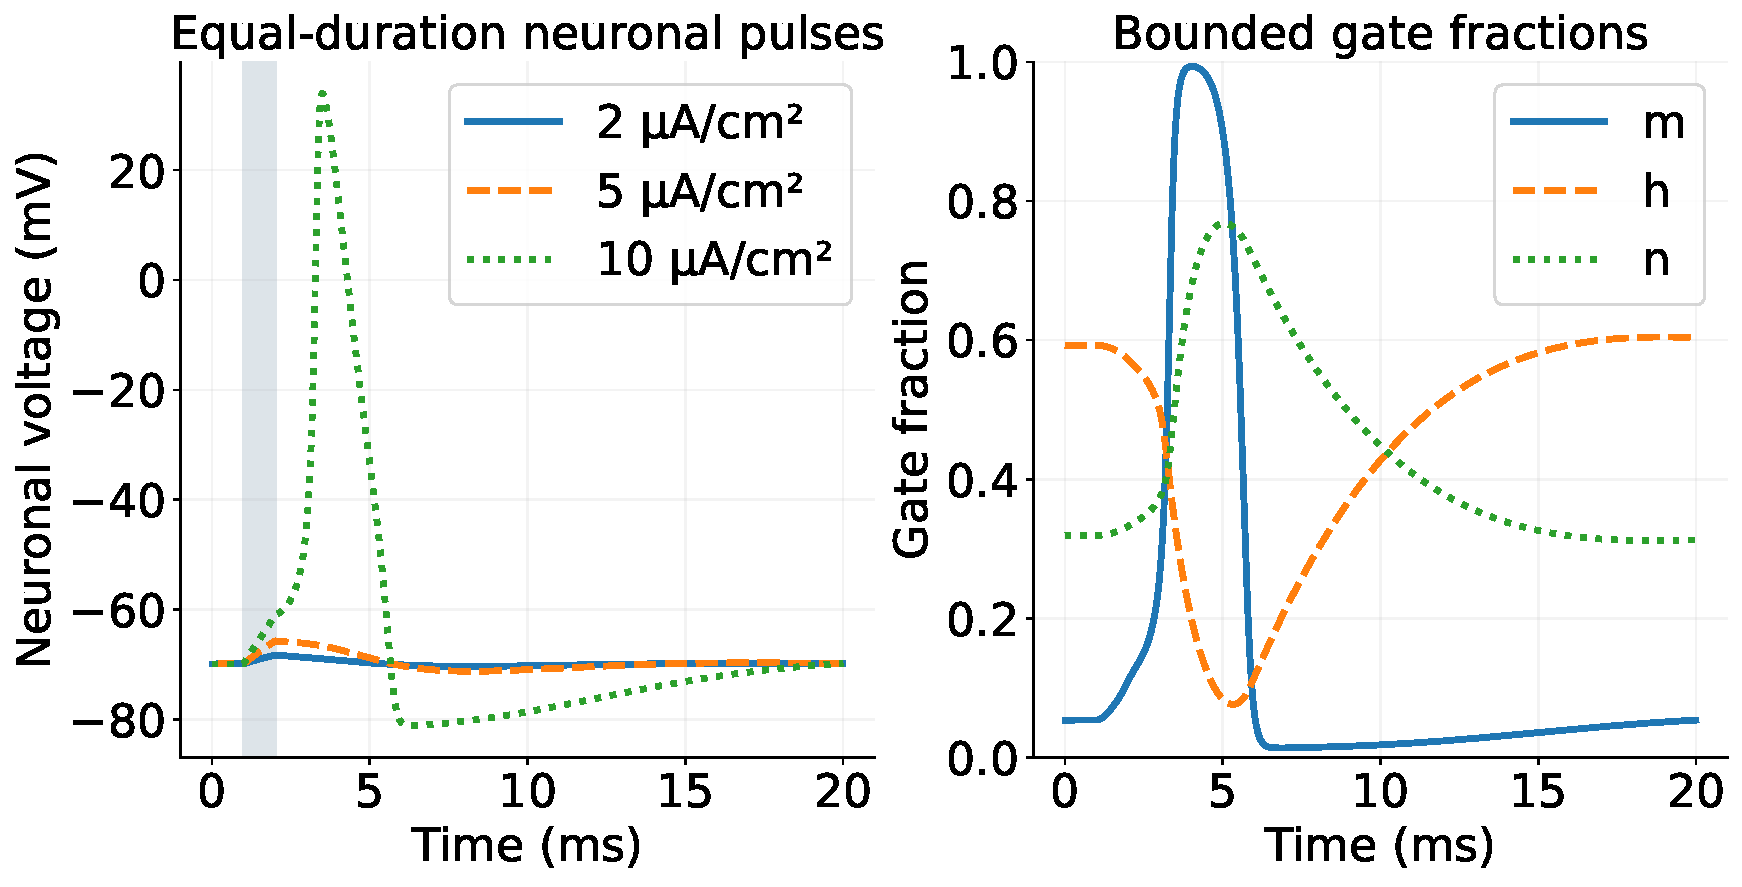
\includegraphics[width=.96\linewidth,height=.57\textheight,keepaspectratio]{neuronal-cell.pdf}\par\smallskip
{\small Original single-cell computations from the current Ahmad neuronal convention. The left panel compares fixed-duration pulses; the right shows the 10 $\mu$A/cm$^2$ gate trajectory. These are not cardiac action potentials.}
\end{minipage}\end{center}
\section{Finite evaluation of the rate functions}
\hypertarget{note-finite-evaluation-of-the-rate-functions}{}\label{note:finite-evaluation-of-the-rate-functions}
{\small \href{slides.html\#frame=the-removable-rate-singularity\&step=1}{Slides for this section}}\par
Two rate expressions contain f(z)=z divided by one minus exp(\ensuremath{-}z). At z=0 both numerator and denominator vanish, although the function has the finite limit one. Evaluating the quotient literally at that point produces an undefined numerical result. Near zero, subtracting two nearly equal floating-point numbers also loses precision. The supplied function uses expm1 away from zero and the local series 1+z/2+z\ensuremath{^{2}}/12\ensuremath{-}z\ensuremath{^{4}}/720 close to zero. This is evaluation of the same continuous function, not a change to the scientific model.

In this convention alpha\_m equals f((V+45)/10), while alpha\_n equals 0.1 times f((V+60)/10). Their removable singularities therefore occur at \ensuremath{-}45 and \ensuremath{-}60 mV, with values 1 and 0.1 per millisecond. The other rates are explicit exponentials or a logistic expression. A useful test includes each exact singular voltage and nearby values from both sides. Checking only a typical resting voltage misses the failure until an excited trajectory crosses the problematic range.

The code validates finite inputs and declares a finite teaching voltage range. It raises an error for invalid data instead of replacing undefined rates with zeros or clipping them. Such replacements would change channel kinetics and can manufacture apparent numerical stability. At the exact singular voltages, the finite rate follows from the analytic limit.

\[
f(z)=\frac{z}{1-e^{-z}},\quad f(0)=1,\quad f(z)=1+\frac z2+\frac{z^2}{12}+O(z^4)
\]
z is dimensionless. The implementation additionally retains the \ensuremath{-}z\ensuremath{^{4}}/720 term.

\[
\alpha_m=f((V+45)/10),\quad\beta_m=4e^{-(V+70)/18}
\]
Voltage V is in mV; all rate values are in ms\ensuremath{^{-1}}.

\[
\alpha_h=0.07e^{-(V+70)/20},\quad\beta_h=\frac{1}{1+e^{-(V+40)/10}}
\]
Use the same voltage convention as both reversal potentials and the other rates.

\[
\alpha_n=0.1f((V+60)/10),\quad\beta_n=0.125e^{-(V+70)/80}
\]
The constants and offsets follow the current Ahmad report.

Expand the denominator as $1-e^{-z}=z-z^2/2+z^3/6-\cdots$ and divide the two power series. The finite continuation is
\[
 f(z)=1+\frac z2+\frac{z^2}{12}-\frac{z^4}{720}+O(z^6).
\]
Away from zero, $f(z)=-z/\operatorname{expm1}(-z)$ avoids forming the difference of two nearly equal numbers. Both expressions evaluate the same rate function.
\section{Exponential gate and voltage substeps}
\hypertarget{note-exponential-gate-and-voltage-substeps}{}\label{note:exponential-gate-and-voltage-substeps}
{\small \href{slides.html\#frame=an-exact-frozen-voltage-gate-step\&step=1}{Slides for this section}}\par
When voltage is held fixed, the gate equation is a linear relaxation. Its exact update is a convex combination of the old fraction and the equilibrium fraction, with exponential weight between zero and one. Nonnegative rates and an admissible old gate therefore imply an admissible new gate for every positive step. There is no need to clip the result. If both rates are zero, the gate remains unchanged. This special case is implemented explicitly through safe division.

Our new integrator first advances all gates with the old voltage. It then freezes their resulting conductances and integrates the linear voltage balance exactly over the same interval. The voltage target is the conductance-weighted reversal potential plus stimulus, divided by total conductance. These two exact frozen subproblems neglect their continuous coupling during the step. The full method is first order, so bounded gates alone cannot certify accurate spike timing or amplitude. This is a different algorithm from the staggered Crank--Nicolson method discussed in the current public report.

A deliberately non-equilibrium initial state makes time error visible. We compare voltage at one millisecond with an independently integrated DOP853 reference, reduce only the step and observe errors approaching a factor of two. The test stays within one smooth stimulus interval. Pulse onset and offset are separate timeline events, including when they are not integer multiples of the nominal step. That prevents refinement from accidentally changing the applied pulse charge.

\[
s^{n+1}=s_\infty+(s^n-s_\infty)e^{-(\alpha+\beta)\Delta t},\quad s_\infty=\frac{\alpha}{\alpha+\beta}
\]
Rates are frozen at the old voltage. The zero-rate case keeps s unchanged.

After the gate substep, let $G=\sum_jg_j$ and $B=\sum_jg_jE_j+I$. With the conductances and stimulus frozen,
\[
 C\dot V=B-GV,\qquad
 V^{n+1}=V_\infty+(V^n-V_\infty)e^{-G\Delta t/C},
 \quad V_\infty=B/G.
\]
The gate and voltage formulas solve their own frozen equations exactly. Their sequential composition does not solve the continuously coupled system exactly: the rates change with $V$ and the conductances change with the gates during each true step.

\paragraph{Calculation.} Freeze alpha=0.2, beta=0.3 ms\ensuremath{^{-1}}, with s=0.9. Compare a one-millisecond update and a large explicit Euler step.

The equilibrium is 0.2/0.5=0.4 and the relaxation time is 2 ms.

At 1 ms the exact value is 0.4+0.5 exp(\ensuremath{-}0.5)=0.703265.

At 5 ms the exact value is 0.4410425. Euler gives 0.9+5(0.2\ensuremath{-}0.5\ensuremath{\times}0.9)=\ensuremath{-}0.35, outside the admissible interval.

Exact frozen-rate evolution preserves the interval; accuracy of the coupled voltage--gate method still requires refinement.
\begin{center}\begin{minipage}{.98\linewidth}\centering
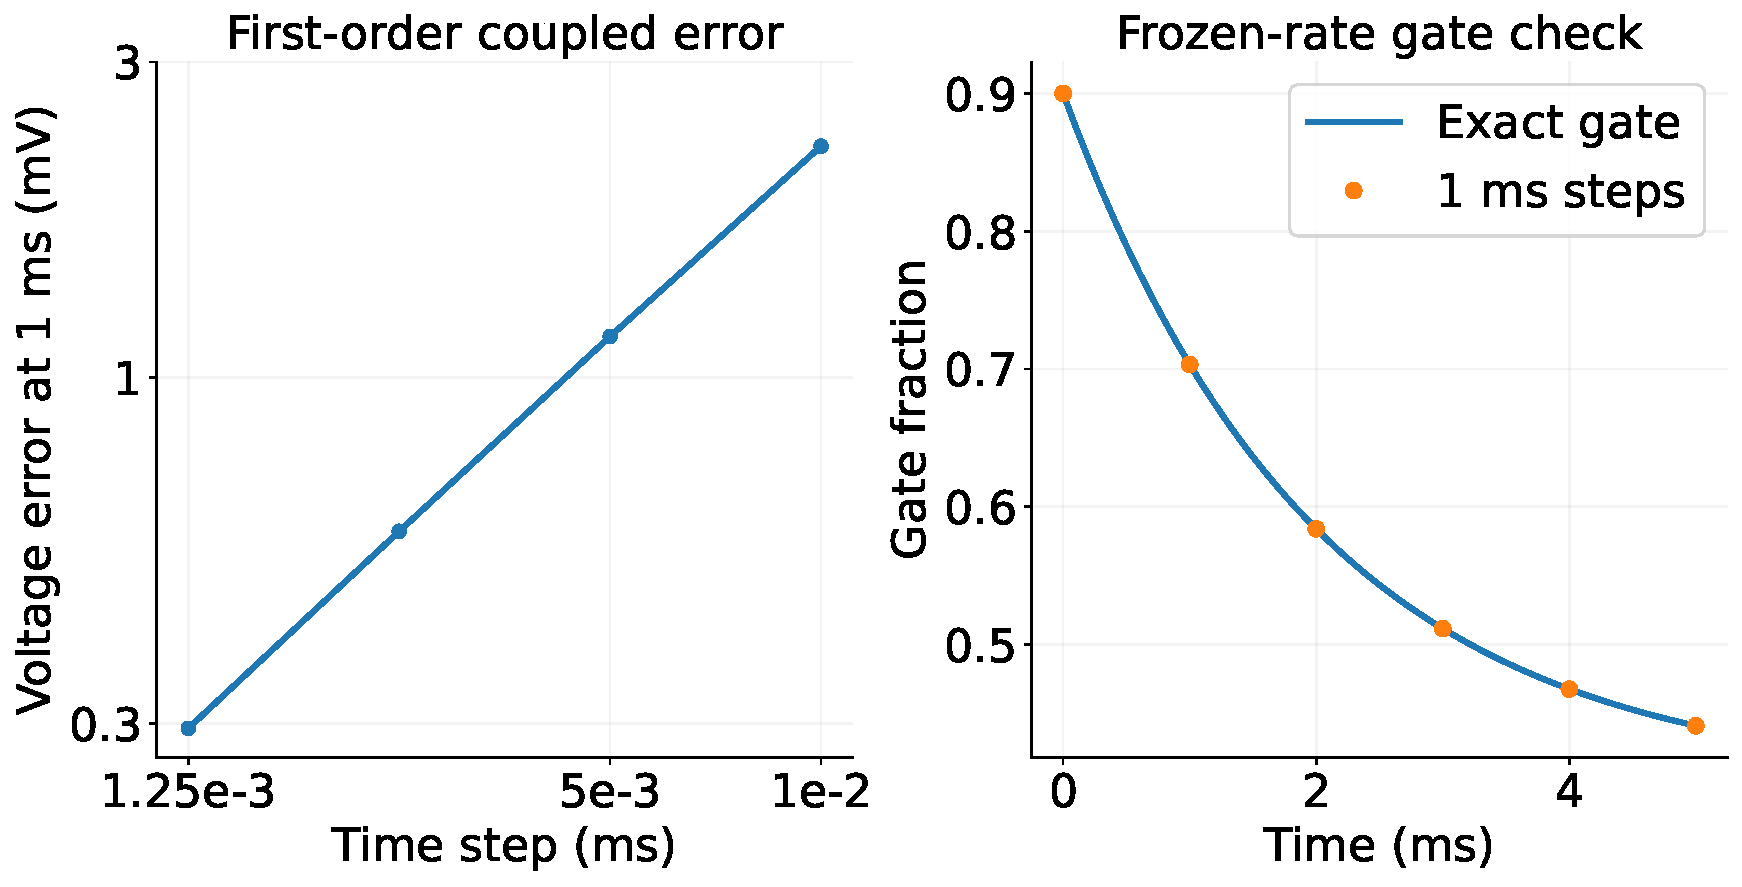
\includegraphics[width=.96\linewidth,height=.57\textheight,keepaspectratio]{gate-and-time-checks.pdf}\par\smallskip
{\small Original independent-reference comparison for the new first-order split solver, alongside an exactly solvable frozen-rate gate. Small-step error approaches first order; the gate solution alone does not validate spike timing.}
\end{minipage}\end{center}
\section{The coupled resting state and stimulus response}
\hypertarget{note-the-coupled-resting-state-and-stimulus-response}{}\label{note:the-coupled-resting-state-and-stimulus-response}
{\small \href{slides.html\#frame=the-coupled-rest-equation\&step=1}{Slides for this section}}\par
A resting state requires more than setting every derivative of voltage to zero by hand. At equilibrium the three gates equal their voltage-dependent equilibrium fractions, and the net ionic current must vanish. We substitute those fractions into the current balance and solve one scalar equation. Using the listed rates and reversal values gives approximately \ensuremath{-}69.8976728964 mV, with a near-roundoff current residual. The printed report gives a nearby rounded value; the companion deliberately recomputes equilibrium from its exact constants rather than claiming both numbers are identical.

Individual ionic currents need not vanish at rest. Opposing currents can balance while charge remains constant. Starting from that coupled state, a zero-stimulus run should preserve voltage and gates to numerical tolerance. A second test changes voltage while retaining the resting gates, which intentionally creates a transient. These tests distinguish a bad initialization from genuine stimulus response and distinguish a numerical drift from relaxation toward an equilibrium.

The supplied comparison applies a one-millisecond pulse starting at one millisecond. With amplitudes 2 and 5 \ensuremath{\mu}A/cm\ensuremath{^{2}} the maximum voltage remains negative, whereas the 10 \ensuremath{\mu}A/cm\ensuremath{^{2}} case makes a large positive excursion. This brackets a response distinction for this initial state and duration; it does not locate a universal threshold. Record the observable you mean by excitation, such as crossing zero, and check whether the conclusion survives time refinement before reporting a threshold search.

The rest voltage is a root of a scalar nonlinear current function:
\[
 \mathcal I(V)=\sum_jg_j(s_\infty(V))(V-E_j)=0.
\]
At this voltage, all gate derivatives and the voltage derivative vanish together. The individual current terms generally do not vanish. A small net current is cancellation of physically signed currents, not evidence that every channel is closed.
\section{Neuronal and reduced cardiac model identities}
\hypertarget{note-neuronal-and-reduced-cardiac-model-identities}{}\label{note:neuronal-and-reduced-cardiac-model-identities}
{\small \href{slides.html\#frame=model-identity\&step=1}{Slides for this section}}\par
The neuronal HH cell is valuable for learning current balance, finite rate functions, competing gates and numerical admissibility. It does not become a ventricular myocyte by changing the title of a plot. A cardiac action-potential model may need a plateau, additional currents, calcium handling, restitution or disease-specific calibration. The appropriate level depends on the observable and the evidence available. Model identity belongs beside every result, especially when code is reused in a new course or tissue geometry.

The two-current reduced cardiac model of Mitchell and Schaeffer uses different variables and kinetics. Its scaled voltage and recovery gate are different state variables from neuronal V, m, h and n. Its aggregate inward and outward terms do not identify individual ionic mechanisms. The transition is a deliberate change of model, not a continuation of the same parameter set. Tissue coupling then introduces another assumption: how local cells exchange current through space.

The state $(V,m,h,n)$ and its listed reversal potentials define the neuronal model used here. The subsequent reduced cardiac system uses a scaled voltage and one aggregate recovery gate. Sharing a gate symbol or a diffusion term does not make the models identical. A plateau, calcium dynamics and tissue-specific calibration require additional equations or parameter evidence.
\bigskip
\section*{Exercises}
\par\noindent\begin{minipage}{\linewidth}
\subsection*{E1. Audit a frozen membrane state}
Use C=\allowbreak{}2 $\mu$F/cm$^2$, V=\allowbreak{}-60 mV and the same reversal values as the notes. Frozen conductances are g\_Na=\allowbreak{}0.01, g\_K=\allowbreak{}0.2 and g\_L=\allowbreak{}0.3 mS/cm$^2$.

\textbf{a} Compute each outward-positive current and their sum.

\end{minipage}\par\medskip
\textbf{b} Find the voltage derivative with an inward stimulus of 1.05 $\mu$A/cm$^2$. State why this is only an instantaneous slope.

\par\noindent\begin{minipage}{\linewidth}
\subsection*{E2. Derive a safe gate update}
Freeze alpha=\allowbreak{}0.3 and beta=\allowbreak{}0.1 ms$^-$$^1$, starting at s=\allowbreak{}0.2.

\textbf{a} Find equilibrium and relaxation time, then evaluate the exact gate after 2 ms.

\end{minipage}\par\medskip
\textbf{b} Compute a single explicit Euler step of 10 ms. Explain the contrast with the exact frozen-rate update.

\par\noindent\begin{minipage}{\linewidth}
\subsection*{E3. Separate implementation checks from biological evidence}
A student reports bounded gates and no NaNs after one pulse.

\textbf{a} Give two additional implementation tests with explicit expected outcomes.

\end{minipage}\par\medskip
\textbf{b} The same student labels the trace a ventricular action potential. Is that supported, and what would support a cardiac claim?

\par\noindent\begin{minipage}{\linewidth}
\subsection*{E4. Design a reproducible excitation comparison}
Two runs use the same initial coupled rest, but one uses a 1 ms pulse and the other a 4 ms pulse.

\textbf{a} Why does comparing their amplitudes alone not identify a common threshold?

\end{minipage}\par\medskip
\textbf{b} Specify a small refinement study that does not change the pulse protocol.

\section*{References}
\noindent\begin{minipage}{\linewidth}
Zan Ahmad, Advanced Topics in Computational Cardiology syllabus, Fall 2024. PDF pages 1--2.

\end{minipage}\par\medskip
\noindent\begin{minipage}{\linewidth}
Hoppensteadt and Peskin, Modeling and Simulation in Medicine and the Life Sciences, second edition. Printed pages 131--134 / supplied PDF pages 144--147: HH rate equations and gate bounds.

\end{minipage}\par\medskip
\noindent\begin{minipage}{\linewidth}
Zan Ahmad, Action Potential Propagation in Branched Neuronal Cables. Current 8-page report, sections 2--3, PDF pages 1--3.

\url{https://zanahmad.com/files/AP_Propagation.pdf}
\end{minipage}\par\medskip
\noindent\begin{minipage}{\linewidth}
Mitchell and Schaeffer, A Two-Current Model for the Dynamics of Cardiac Membrane (2003). Printed pages 769--772; author-hosted PDF pages 3--6, equations 1--5 and Figure 1 parameters.

\url{https://homepage.divms.uiowa.edu/~mtchll/2Current.pdf}
\end{minipage}\par\medskip
\end{document}
